\documentclass[crop,tikz,convert={density=300,size=1080x1080,outext=.png}]{standalone}
\usepackage{physics}
\usetikzlibrary{positioning}
\usetikzlibrary{arrows}

\begin{document}
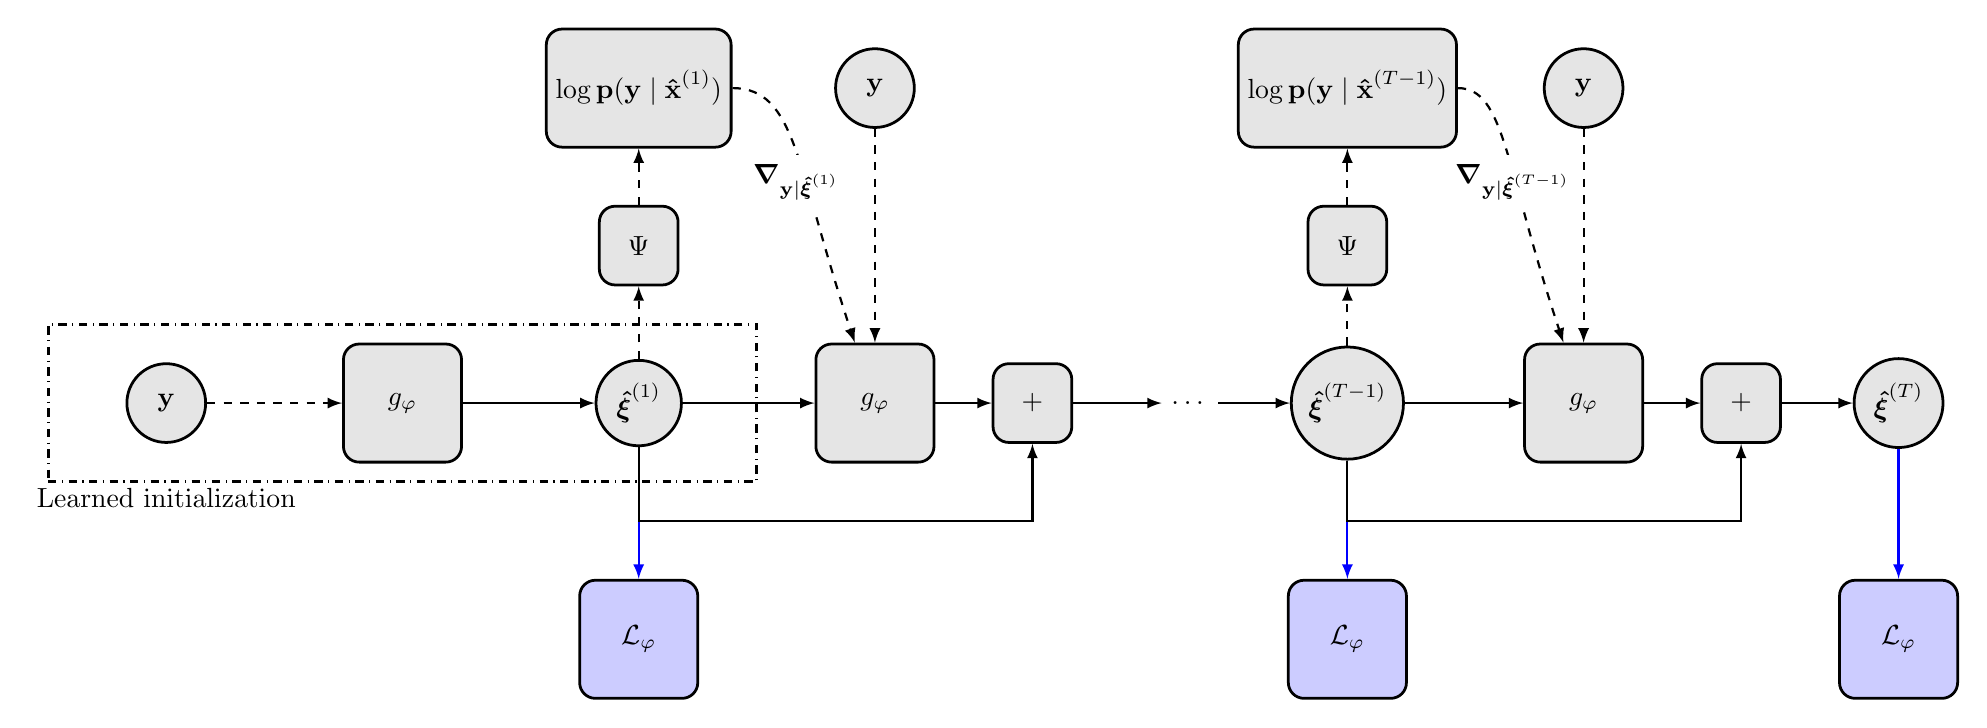
\begin{tikzpicture}[
        node/.style={shape=rectangle, minimum size=1.5cm, rounded corners=.2cm, draw=black, line width=1, fill=black!10},
        op/.style={shape=rectangle, minimum size=1cm, rounded corners=.2cm, draw=black, line width=1, fill=black!10},
        var/.style={shape=circle, minimum size=1cm, draw=black, line width=1, fill=black!10},
edge/.style={-latex, thick},
node distance=3cm,
every text node part/.style={align=center}
]
\node[var] (y) at (0, 0) {$\mathbf{y}$};
\node[node] (g1) at (3, 0) {$g_\varphi$};
\draw[edge, dashed] (y) to (g1);
\node[shape=rectangle, minimum height=2cm, minimum width=9cm, dash dot, draw=black, line width=1] at (3, 0) {}; 
\node at (0, -1.2) {Learned initialization};

\node[var] (x1) at (6, 0) {$\boldsymbol{\hat{\xi}}^{(1)}$};
\node[node, fill=blue!20] (l1) at (6, -3) {$\mathcal{L}_{\varphi}$};
\draw[edge, blue] (x1) to (l1);
\draw[edge] (g1) to (x1);
\node[node] (g2) at (9, 0) {$g_\varphi$};
\node[op] (psi1) at (6, 2) {$\Psi$};
\node[node] (p1) at (6, 4) {$\log \mathbf{p(\mathbf{y} \mid \mathbf{\hat{x}}}^{(1)})$};
\draw[edge, dashed] (p1) .. controls +(2, 0) and +(-1, 3) .. (g2);
\node[fill=white] at (8, 2.8) {$\grad_{\mathbf{y} \mid \boldsymbol{\hat{\xi}}^{(1)}}$};
\draw[edge, dashed] (x1) to (psi1);
\draw[edge, dashed] (psi1) to (p1);
\draw[edge] (x1) to (g2);
%\node[var] (y1) at (6, 6) {$\mathbf{y}$};
%\draw[edge, dashed] (y1) to (p1);
\node[var] (y2) at (9, 4) {$\mathbf{y}$};
\draw[edge, dashed] (y2) to (g2);

\node[var] (x2) at (15, 0) {$\boldsymbol{\hat{\xi}}^{(T-1)}$};
\node[node, fill=blue!20] (l2) at (15, -3) {$\mathcal{L}_{\varphi}$};
\draw[edge, blue] (x2) to (l2);
\node (dots) at (13, 0) {$\dots$};
\node[op] (plus) at (11, 0) {$+$};
\draw[edge] (x1) -- ++(0, -1.5) -- ++(5, 0) -- (plus);
\draw[edge] (g2) to (plus);
\draw[edge] (plus) to (dots);
\draw[edge] (dots) to (x2);
\node[node] (g3) at (18, 0) {$g_\varphi$};
\node[op] (psi2) at (15, 2) {$\Psi$};
\node[node] (p2) at (15, 4) {$\log \mathbf{p(\mathbf{y} \mid \mathbf{\hat{x}}}^{(T-1)})$};
\draw[edge, dashed] (p2) .. controls +(2, 0) and +(-1, 3) .. (g3);
\node[fill=white] at (17.1, 2.8) {$\grad_{\mathbf{y} \mid \boldsymbol{\hat{\xi}}^{(T-1)}}$};
\draw[edge, dashed] (x2) to (psi2);
\draw[edge, dashed] (psi2) to (p2);
\draw[edge] (x2) to (g3);
%\node[var] (y3) at (15, 6) {$\mathbf{y}$};
%\draw[edge, dashed] (y3) to (p2);
\node[var] (y3) at (18, 4) {$\mathbf{y}$};
\draw[edge, dashed] (y3) to (g3);
\node[var] (xT) at (22, 0) {$\boldsymbol{\hat{\xi}}^{(T)}$};
\node[op] (plus2) at (20, 0) {$+$};
\draw[edge] (g3) to (plus2);
\draw[edge] (x2) -- ++(0, -1.5) -- ++(5, 0) -- (plus2);
\draw[edge] (plus2) to (xT);
\node[node, fill=blue!20] (lT) at (22, -3) {$\mathcal{L}_{\varphi}$};
\draw[edge, blue] (xT) to (lT);


\end{tikzpicture}
\end{document}
